% ****** Start of file apssamp.tex ******
%
%   This file is part of the APS files in the REVTeX 4.2 distribution.
%   Version 4.2a of REVTeX, December 2014
%
%   Copyright (c) 2014 The American Physical Society.
%
%   See the REVTeX 4 README file for restrictions and more information.
%
% TeX'ing this file requires that you have AMS-LaTeX 2.0 installed
% as well as the rest of the prerequisites for REVTeX 4.2
%
% See the REVTeX 4 README file
% It also requires running BibTeX. The commands are as follows:
%
%  1)  latex apssamp.tex
%  2)  bibtex apssamp
%  3)  latex apssamp.tex
%  4)  latex apssamp.tex
%
\documentclass[%
reprint,
superscriptaddress,
%groupedaddress,
%unsortedaddress,
%runinaddress,
%frontmatterverbose, 
%preprint,
%preprintnumbers,
%nofootinbib,
%nobibnotes,
%bibnotes,
amsmath,amssymb,
aps,
%pra,
prb,
%rmp,
%prstab,
%prstper,
%floatfix,
]{revtex4-2}

\usepackage{graphicx}% Include figure files
\usepackage{dcolumn}% Align table columns on decimal point
\usepackage{bm}% bold math
\usepackage{physics}
\usepackage{natbib}
\usepackage{epsfig}
\usepackage{epstopdf}
\usepackage{dsfont}

\usepackage{hyperref}
\usepackage[usenames,dvipsnames]{xcolor}
\hypersetup{colorlinks, linkcolor={red},citecolor={blue}, urlcolor={MidnightBlue}}

%\usepackage{hyperref}% add hypertext capabilities
%\usepackage[mathlines]{lineno}% Enable numbering of text and display math
%\linenumbers\relax % Commence numbering lines

%\usepackage[showframe,%Uncomment any one of the following lines to test 
%%scale=0.7, marginratio={1:1, 2:3}, ignoreall,% default settings
%%text={7in,10in},centering,
%%margin=1.5in,
%%total={6.5in,8.75in}, top=1.2in, left=0.9in, includefoot,
%%height=10in,a5paper,hmargin={3cm,0.8in},
%]{geometry}

\begin{document}
	
	\preprint{APS/123-QED}
	
	\title{Eccentric Phase Transition from Thermalization to Many Body Localization  in Long-Range Spin Systems using Floquet Engineering}% Force line breaks with \\
	%\thanks{A footnote to the article title}%
	
	\author{Mahbub Rahaman}
	\affiliation{Department of Physics, The University of Burdwan, Golapbag, Bardhaman - 713 104, India}
	\author{Takashi Mori}
	\affiliation{RIKEN CEMS, 2-1 Hirosawa, Wako, Saitama, 351-0198, Japan}
	\author{Analabha Roy}
	\affiliation{Department of Physics, The University of Burdwan, Golapbag, Bardhaman - 713 104, India}
	
	\begin{abstract}
		Many-body localization is a  quantum phenomenon where a quantum system retains its initial state under certain resonance conditions, $J_0(\eta)$ which prevents the system to undergo thermalization. We have validated many-body localization for spin systems driven by transverse field and parametrized it by the Inverse Participation ratio(IPR) of Floquet modes. Long-range power-law dependence $i.e.$ $J_{ij} = 1/|i-j|^{\beta}$ has been applied and we investigated for $\beta = \infty$ for short-range Transverse Field Ising Model and for  $\beta = 0$  long-range Lipkin Meshkov-Glick (LMG) model is explored both at low and high drive frequencies. At the localization point Ising model exhibit full localisation at  high frequency though at low-frequency localization persists. For the long-range case, at the system localization point, LMG shows localization at high frequency though at smaller frequency localization breaks down with inverse system size law. Similar behaviour is found in LMG at the phase-space continuum limit where at low-frequency chaos emerges and at the higher frequency it is regular. IPR for LMG is evolved by an adiabatic increase in drive frequencies; the IPR rises sharply  thereby introducing a phase transition which manifests a future protocol for the MBL engine.
		
		%\begin{description}
		%\item[Usage]
		%Secondary publications and information retrieval purposes.
		%\item[Structure]
		%You may use the \texttt{description} environment to structure your %abstract;
		%use the optional argument of the \verb+\item+ command to give the %category of each item. 
		%\end{description}
	\end{abstract}
	
	\keywords{Phase transition, Long range interaction, Many body localiszation}%Use showkeys class option if keyword
	%display desired
	\maketitle
	
	%\tableofcontents
	
	NEED TO PROOFREAD THIS. WILL DO AT THE END.
	
	Periodically driven Many Body Systems can experience dynamical freezing (DMF) when a dynamical hysteresis stops observables from reaching their diagonal averaged values and thermalizing to infinite temperature ~\cite{bordia_periodically_2017, sahoo_periodically_2019, das_exotic_2010}. Under certain resonance conditions in the drive parameters, DMF can cause the response to ‘freeze’ completely to its initial value at all times. This has been demonstrated via the Jordan-Wigner (JW) transformation in the driven TFIM with nearest neighbour interactions ~\cite{mbeng_quantum_2020} and is shown to be protected when translational invariance is explicitly broken (say, by disorder) ~\cite{yamada_localization_2022, roy_fate_2015}. 
	
	We have a hunch that this symmetry is preserved against the loss of other symmetries such as Long-range systems for which the JW transformation results in nonlocalities. To prove this, we introduce a long-range power-law dependence in the TFIM, where the exchange $J_{ij}\sim 1/|i-j|^\beta$; for $\beta=\infty$ ~\cite{campa_statistical_2009, eisele_multiple_1988, canning_class_1992}, we recover the short-range TFIM and freezing at resonant drive parameters. When $\beta=0$, taking $N\rightarrow\infty$ allows us to describe the exact dynamics by the periodically driven Lipkin-Meshkov-Glick (LMG) model.
	
	Now, we compare the degree of localization of the quasi-stationary Floquet modes in both cases. In order to do so, we look at the Inverse Participation Ratio (IPR) of the Floquet modes in the representation given by the eigenstates of the symmetry-breaking field. The Inverse Participation Ratio (IPR) ~\cite{Misguich2016} a parameter is a useful tool for defending the many-body localization of a quantum system. For a many-body localized system, IPR is unity and it varies as the inverse of the system size when it is fully distributed ~\cite{calixto_inverse_2015}.
	
	In the first section of this paper, we presented a brief overview of essential theoretical frameworks. The Ising Model driven by a transverse periodic field which breaks symmetry is presented next in section II. Rotating Wave Approximation (RWA) ~\cite{fujii_introduction_2017}, where only the slowest rotating terms in the Fourier expansion of the Hamiltonian in a frame co-rotating with symmetry breaking drive field are retained, is used to make a close approximation of the Ising Hamiltonian, and higher-order corrections are obtained also. We have applied the Floquet theory of a periodically driven system and obtained Floquet modes to get the IPR of the Floquet modes. It is used to probe the system dynamics in the high and low-frequency domains. In section III we introduce  LMG model as a paradigmatic spin model for long-range spin-spin interaction. We formulated the system Hamiltonian which governs it at a continuum limit and also simplified it using RWA to find Floquet-IPR for low and high-frequency regions of operation. In section IV we have contrasted the classical Lipkin model driven with both at a higher frequency and sufficient lower frequency for phase-space and Hushimi Q-functions analysis. In section V we have discussed the  system dynamics driven by adiabatically increased drive frequency from low to high limit thereby we discover a phase transition at the system localization resonance point. Finally, we conclude and discuss the outlook. 
	
	\section{\label{sec:background} Background}
	
	PROOFREADING THIS NOW.
	
The Floquet Eigenstate Thermalization Hypothesis (FETH) is a theoretical construct that characterizes the thermalization process of a quantum system that is subject to a time-periodic many-body Hamiltonian. The framework presented enables comprehension of the thermal-like behavior exhibited by a system that is intrinsically out of equilibrium. The Floquet Engineering Theorem (FETH) holds significant relevance in the investigation of stimulated quantum systems, wherein the Hamiltonian undergoes periodic fluctuations over time.

To understand FETH, let's consider a many-body system described by a time-periodic Hamiltonian H(t) with a period T. The time evolution of the system is governed by the Schrödinger equation, $i\hbar \frac{\partial{\psi(t)}}{\partial{t}} = H(t)\psi(t)$, where $\psi(t)$ is the state vector of the system at time t.

The Floquet theorem states that for a time-periodic Hamiltonian, the solutions of the Schrödinger equation can be written as $\psi(t) = e^{-i\epsilon t/\hbar} \phi(t)$, where $\phi(t)$ is a T-periodic function and$\epsilon$ is the quasienergy. The quasienergy spectrum is bounded within a range of $[-\hbar\omega/2, \hbar\omega/2]$, where $\omega = 2\pi/T$ is the driving frequency.

According to FETH, in the limit of large system size and under certain conditions, the quasienergy eigenstates of the time-periodic Hamiltonian behave like thermal states. Specifically, for an observable A, the expectation value of A in a quasienergy eigenstate $\psi_\alpha$ with quasienergy $\epsilon_\alpha$ can be approximated by the thermal expectation value:
\begin{equation}
\bra{\psi_\alpha}\hat{A}\ket{\psi_\alpha} = \frac{Tr (Ae^{-\beta H_{eq}})}{Tr(e^{-\beta H_{eq}})}
\end{equation}
 
where $\beta = 1/(k_B T)$ is the inverse temperature, $H_{eq}$ is an effective Hamiltonian that captures the long-time average dynamics of the system, and $k_B$ is the Boltzmann constant.

In summary, FETH suggests that the time-periodic many-body Hamiltonian exhibits thermalization in the long-time limit, with the quasienergy eigenstates resembling thermal states. This hypothesis provides a valuable tool for understanding the behavior of driven quantum systems and their connection to thermal equilibrium.


The Eigenstate Thermalization Hypothesis (ETH) is a conjecture that relates the expectation values of observables in individual eigenstates of a quantum system to the predictions of statistical mechanics. The derivation of ETH involves the assumption of ergodicity, which states that a system explores all accessible states in its phase space uniformly over time.
Consider a many-body quantum system described by a time-dependent periodic Hamiltonian H(t) with a period T. The Schrödinger equation governing the time evolution of the system is given by $i\hbar \pdv{\psi(t)}{t} = \hat{H}(t) \ket{\psi(t)}$

$i\hbar \pdv{\psi(t)}{t} = H(t) \ket{\psi(t)}$, where $\ket{\psi(t)}$ is the state vector of the system at time t. We aim to derive ETH by examining the expectation value of an observable A in an eigenstate of the Hamiltonian.

Let $\ket{n(t)}$ be an eigenstate of H(t) with energy $E_n (t)$, such that $H(t)\ket{n(t)} = E_n (t)\ket{n(t)}$. We want to calculate the expectation value of the observable A in this eigenstate: $\expval{\hat{A}(t)}_n = \expval{\hat{A}(t)}{{n(t)}}$.

To proceed with the derivation, we invoke the concept of adiabatic perturbation theory, assuming that the Hamiltonian slowly varies in time. We can expand the eigenstate and eigenenergy as perturbative series:
\begin{align*}
\ket{n(t)} =& \ket{n(\theta)} + \sum_m c_m(t)\ket{m(\theta)},\\ 
E_n (\theta) =& E_n (\theta) + \sum_m E_m (t) c_m(t)
\end{align*}
where $\ket{m(\theta)}$ represents the unperturbed eigenstates of $H(\theta)$ with energy $E_m(\theta)$. The coefficients $c_m (t)$ describe the time-dependent amplitude of the expansion.
Plugging these expansions into the expression for the expectation value, we obtain:
\begin{widetext}
\expval{\hat{A}(t)}_n = \sum_{m,k} c_M^*(t) c_k(t) \bra{n(\theta)}\ket{m(\theta}\bra{m(t)}\hat(A)(t)\ket{k(t)} \bra{k(\theta)}\ket(n(\theta))
\end{widetext}
where $ \bra{m(t)}\hat(A)(t)\ket{k(t)}$ represents the matrix element of the observable $\hat{A}$ between the time-dependent states $\ket{m(t)}$ and $\ket{k(t)}$.
In the ergodic hypothesis, it is assumed that the system explores the entire Hilbert space uniformly, such that the matrix elements ⟨m(t)|A(t)|k(t)⟩ become indistinguishable for most pairs of m and k. This allows us to approximate $\bra{m(t)}\hat{A}(t)\ket{k(t)} ≈ A_{eq} \delta_{mk}$, where $A_{eq}$ is the expectation value of the observable $\hat{A}$ in the equilibrium thermal ensemble.
Applying this approximation, the expression for the expectation value becomes:
\begin{equation*}
\expval{\hat{A}(t)}_n = \sum_m \abs{c_m(t)}^2 \bra{n(\theta)}\ket{m(\theta)} \hat{A}_{eq} \bra{n(0)}\ket{m(0)}
\end{equation*}
Finally, assuming that the initial state |n(0)⟩ is random and uncorrelated with the Hamiltonian eigenstates, we can use the property $\bra{n(0)}\ket{m(0)}=\delta_{nm}$. This yields:
\begin{equation*}
\expval{\hat{A}(t)}_n = \sum_m |c_m(t)|^2 \hat{A}_{eq} = \hat{A}_{eq}
\end{equation*}
Therefore, in the limit of large systems and under the ergodic assumption, the expectation value of an observable A in an eigenstate of the time-dependent Hamiltonian is approximately equal to the thermal expectation value $A_{eq}$. This is the essence of the Eigenstate Thermalization Hypothesis, which suggests that individual eigenstates of a quantum system can be described by statistical mechanics in the long-time limit.
	
	A paradigmatic example of an integrable system where DMBL occurs is  the driven Transverse Field Ising model (TFIM) in one dimension~\cite{stinchcombe_ising_1973}. The Hamiltonian is given by
	\begin{align}
		\label{eq:tfim:hamilt}
		\hat{H}(t) &= \hat{H}_0 + h_z(t) \; \hat{H}_1\\
		\hat{H}_0 &= -\frac{1}{2}\sum^N_{i=1} \sigma^x_i \sigma^x_{i+1}\\
		\hat{H}_1 &= -\frac{1}{2}\sum_{i=1}^N \sigma^z_{i}.
	\end{align}
	Here, the undriven Hamiltonian $\hat{H}_0$ consists of nearest-neighbour itneractions between $N$ spin-$1/2$ particles on a one-dimensional lattice. The transverse field is given by $\hat{H}_1$, and is being modulated by a time-periodic and harmonic signal $h_z(t) = h_0 + h\cos{\omega t}$, yielding a time period $T=2\pi/\omega$ with amplitude $h$, drive frequency $\omega$, and d.c. field $h_0$. This Hamiltonian can be readily transformed into a spinless pseudo-fermionic system via the Jordan-Wigner transformation. Written in momentum space spanned by spinors $\psi_k = (c_{-k}, c^\dagger_k)^T$ of fermions at momentum $k$ created (annihilated) by operators $c^\dagger_k$ ($c_k$). This yields an effective Hamiltonian ~\cite{mbeng_quantum_2020}
	\begin{equation}
		H(t) = \sum_{(k,-k)-\mbox{pairs}} \psi^\dagger_k
		\Bigg[\ \bigg(f_k - h_z(t)\bigg)\tau_z +  \tau_x \Delta_k\Bigg]\psi_k
	\end{equation}
	with $f_k = J\cos{k}$, $\Delta_k = J\sin{k}$, $\tau_{xyz}$ are the three Pauli Matrices, and the sum is over distinct $(k, -k)$ \textit{Cooper Pairs}. Now, we transform to the rotated frame via the unitary transformation operator $U(t) = \prod_k U_k(t)$, where $U_k(t) = \exp{\Big[\frac{i h}{\omega}\sin{\omega t}\Big]\tau_z}$. This yields the transformed Hamiltonian
	\begin{multline*}
		H^\prime(t) = \sum_{(k,-k)-\mbox{pairs}} \psi^\dagger_k
		\bigg[\ \tau_z f_k + \tau_x \cos{\big(\eta\sin{\omega t}\big)}  \\
		+ \tau_y \cos{\big(\eta\sin{\omega t}\big)}\bigg]\psi_k,
	\end{multline*}
	where we defined $\eta=2h/\omega$. Using the Jacobi-Anger formula $e^{i \eta \sin{\omega t}} = \sum_{n=-\infty}^{\infty} J_n(\eta)\, e^{i n \omega t}$, the transformed Hamiltonian simplifies to \\
	\begin{align}
		H^\prime(t) =& \sum_{(k,-k)-\mbox{pairs}} \psi^\dagger_k
		\bigg[\ \tau_z f_k + 2\tau_x \Delta_k \sum_{n\geq 0} J_{2n}(\eta)\cos{\big(2n\omega t\big)} \nonumber\\
		&\hskip 1.2cm- 2\tau^y\Delta_k \sum_{n\geq 0} J_{2n+1}(\eta)\sin{\big\{\big(2n+1\big)\omega t\big\}}   \bigg]\psi_k,
	\end{align}\\
	Now, for large $\omega \gg f_k$, we can approximate $H^\prime(t)$ by its long-time average $\overline{H^\prime(t)}$, leaving behind only the non-oscillating modes, a  \textit{Rotated Wave Approximation} that yields an effective time-independent Hamiltonian,
	\begin{equation}
		\label{eq:hrwa:tfim}
		H^{RWA} = \sum_{(k,-k)-\mbox{pairs}} \psi^\dagger_k
		\bigg[\ f_k\tau_z + 2 J_0(\eta) \Delta_k\tau_x \bigg]\psi_k,
	\end{equation}
	Clearly, if we engineer drive parameters such that $\eta$ lies on a root of $J_0(\eta)$, a straightforward case of Floquet Engineering, then the fermion number (THIS PART STILL NEEDS WORK) becomes an approximately conserved quantity at this resonance. Thus, it is possible to directly control $H^{RWA}$ and induce a complete freezing of otherwise responsive observables. That this leads to a spectacular breakdown of ETH can be readily demonstrated by ... NOW CONTEXUALIZE THIS WRT THE DREK ABOUT FUNCTIONAL DERIVATIVES...
	
	The extent to which a particular (quasi) stationary state is localized (or frozen) in a physically meaningful representation can be quantified by the \emph{Inverse Participation Ratio} (IPR). In the position representation, the IPR for a state $\ket{\psi}$  \cite{mukherjee_modulation-assisted_2015,lin_many-body_2018,murphy_generalized_2011, torres-herrera_self-averaging_2020} is defined as
	\begin{equation*}
		\phi_{IPR}\equiv \int \mathrm{d}\mathbf{x}\;\vert\ip{\mathbf{x}}{\psi}\vert^4
	\end{equation*}
	This definition can be generalized to the IPR of a state $|\phi\rangle$ in a representation given by complete orthonormal basis $\ket{m}$ as 
	\begin{equation}
	\label{eq:ipr:defn}
	\phi_{IPR} \equiv \sum_m\vert\ip{m}{\psi}\vert^4.
	\end{equation}
	The smallest value of the IPR corresponds to a fully delocalized state, $\psi(x)=1/\sqrt{N}$ for a system of size $N$ \cite{torres-herrera_self-averaging_2020,trivedi_can_2005}. Values of the IPR close to unity correspond to localized states \cite{misguich_inverse_2016}. For a periodically driven system, we look at the IPR of the quasi-stationary Floquet modes at $t=T$, where $t=2\pi/\omega$ for drive frequency $\omega$. In the TFIM model, equation~\ref{eq:hrwa:tfim} indicates that, at resonance, when $J_0(\eta)=0$, the Floquet modes are approximately given by the fermionic Fock states, which have a trivially unit IPR in the representation of the eigenmodes of the transverse field $\hat{H}_1$ in equation~\ref{eq:tfim:hamilt}.
		
	For the TFIM case,  a particular Floquet mode can be decomposed into a direct product of cooper-pair states as $|\phi\rangle = \prod_{k,-k}|\phi^n_k\rangle$. In the RWA limit and at resonance, $|\phi^n_k\rangle$ has values of $|0\rangle, |k,-k\rangle$ for two values of $n=0,1$ respectively. We define the reduced IPR of $|\phi^n_k\rangle\; \forall k$ to be
	\begin{equation}
	\label{eq:ipr:ising}
	\phi^{(n)}_{IPR}(k) = \abs{\ip{0}{\phi^n_k}}^4 + \abs{\ip{ +k, -k }{\phi^n_k}}^4,
	\end{equation}
	where $n=0,1$. In the RWA limit and at resonance , this quantity is unity, indicating very low participation and the onset of freezing.
	\begin{figure}[hbt!]
		\centering
		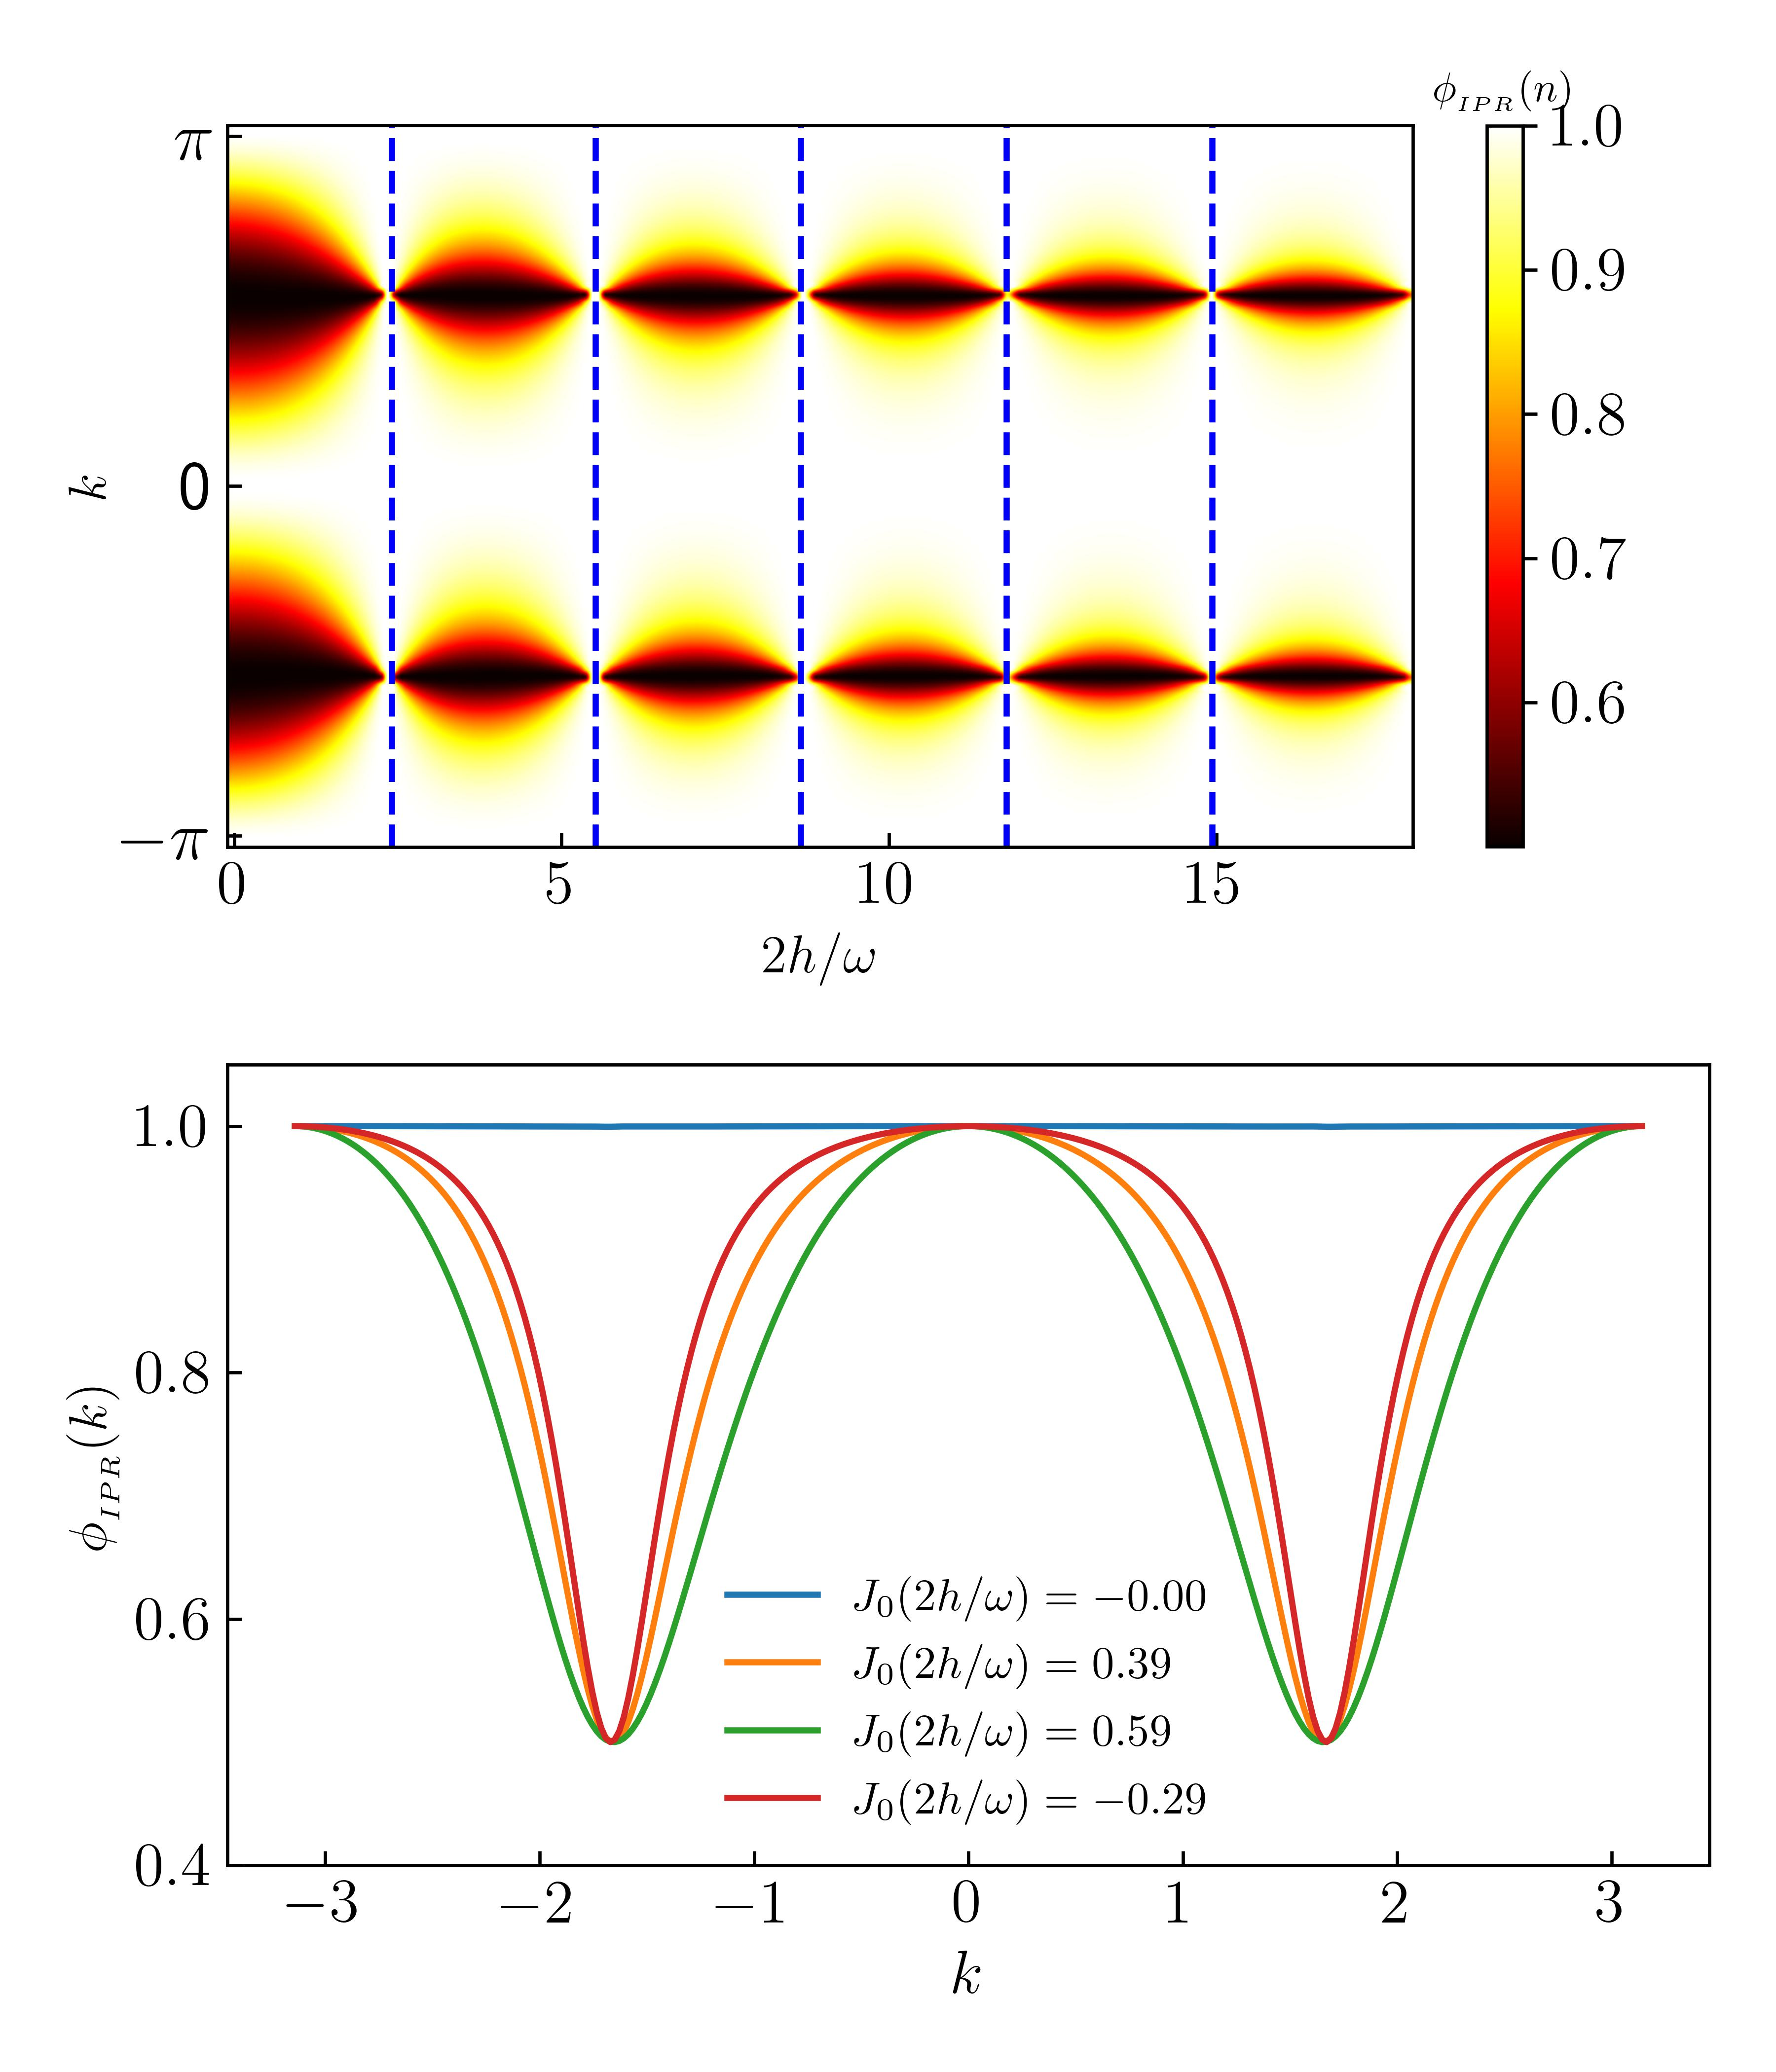
\includegraphics[height = 10cm, width = 9.0cm]{ising_exact_ipr.jpeg}
		\caption{The plots above are for the exact dynamics of the TFIM in Fermionic representation for size N = 100, with the reduced IPR (defined in equation~\ref{eq:ipr:ising}) plotted for the entire Brillouin zone for a few drive amplitudes. The frequency is set to $\omega = 90$ and the IPR of one of the two Floquet modes are plotted at time $t=T$ for four different chosen amplitudes. The exact result is consistent with the RWA approximation. When $J_0(2h/\omega) = 0$, the RWA Hamiltonian vanishes, yielding an IPR of unity. At other points, the IPR is unity only when $k=\pm \pi$ (since $\Delta_k=0$) and $k=0$ (since $f_k = 0$ and the Hamiltonian for each $k$ $\sim \sigma_x$); other than that, there is freezing due to the ensuing dynamics.}
		\label{fig:ipr:tfim}
	\end{figure}
	Figure~\ref{fig:ipr:tfim} shows results from numerically simulating the TFIM dynamics. The reduced IPR for a particular Floquet mode was obtained by simulating the exact Heisenberg dynamics over a single time period of the drive, and plotted as a function of momentum $k$ for different $\eta$'s. At resonance, when $\eta$ lies at the root of the Bessel function $J_0(\eta)$,  the IPR is exactly unity for all momenta. Outside this resonance, the IPR is unity only for some momenta because the effective Hamiltonian is perfect diagonal at $k \in{\{-\pi, 0, \pi\}}$ as can be seen in the cross-sectional plots of figure~\ref{fig:ipr:tfim}. Away from the resonance point, IPR is less than unity but as TFIM is integrable spin model, it does not follow thermalization maintaining posetive value. However, at low frequencies, when RWA fails due to unavailibity of zero offdiagonal terms in the  effective transformed Hamiltonian (in matrix representation) and no integrability breaking terms to counteract the off diagonal terms, the IPR remains quite high ($IPR \sim 0.5$) even at resonance point as can be seen figure~\ref{fig:ipr:isinglowfr}. At low frequency, this is valid for all momentum and parameter $\eta$, see figure~\ref{fig:ipr:isinglowfrk}.
	
	
	
	\begin{figure}[hbt!]
		\centering
		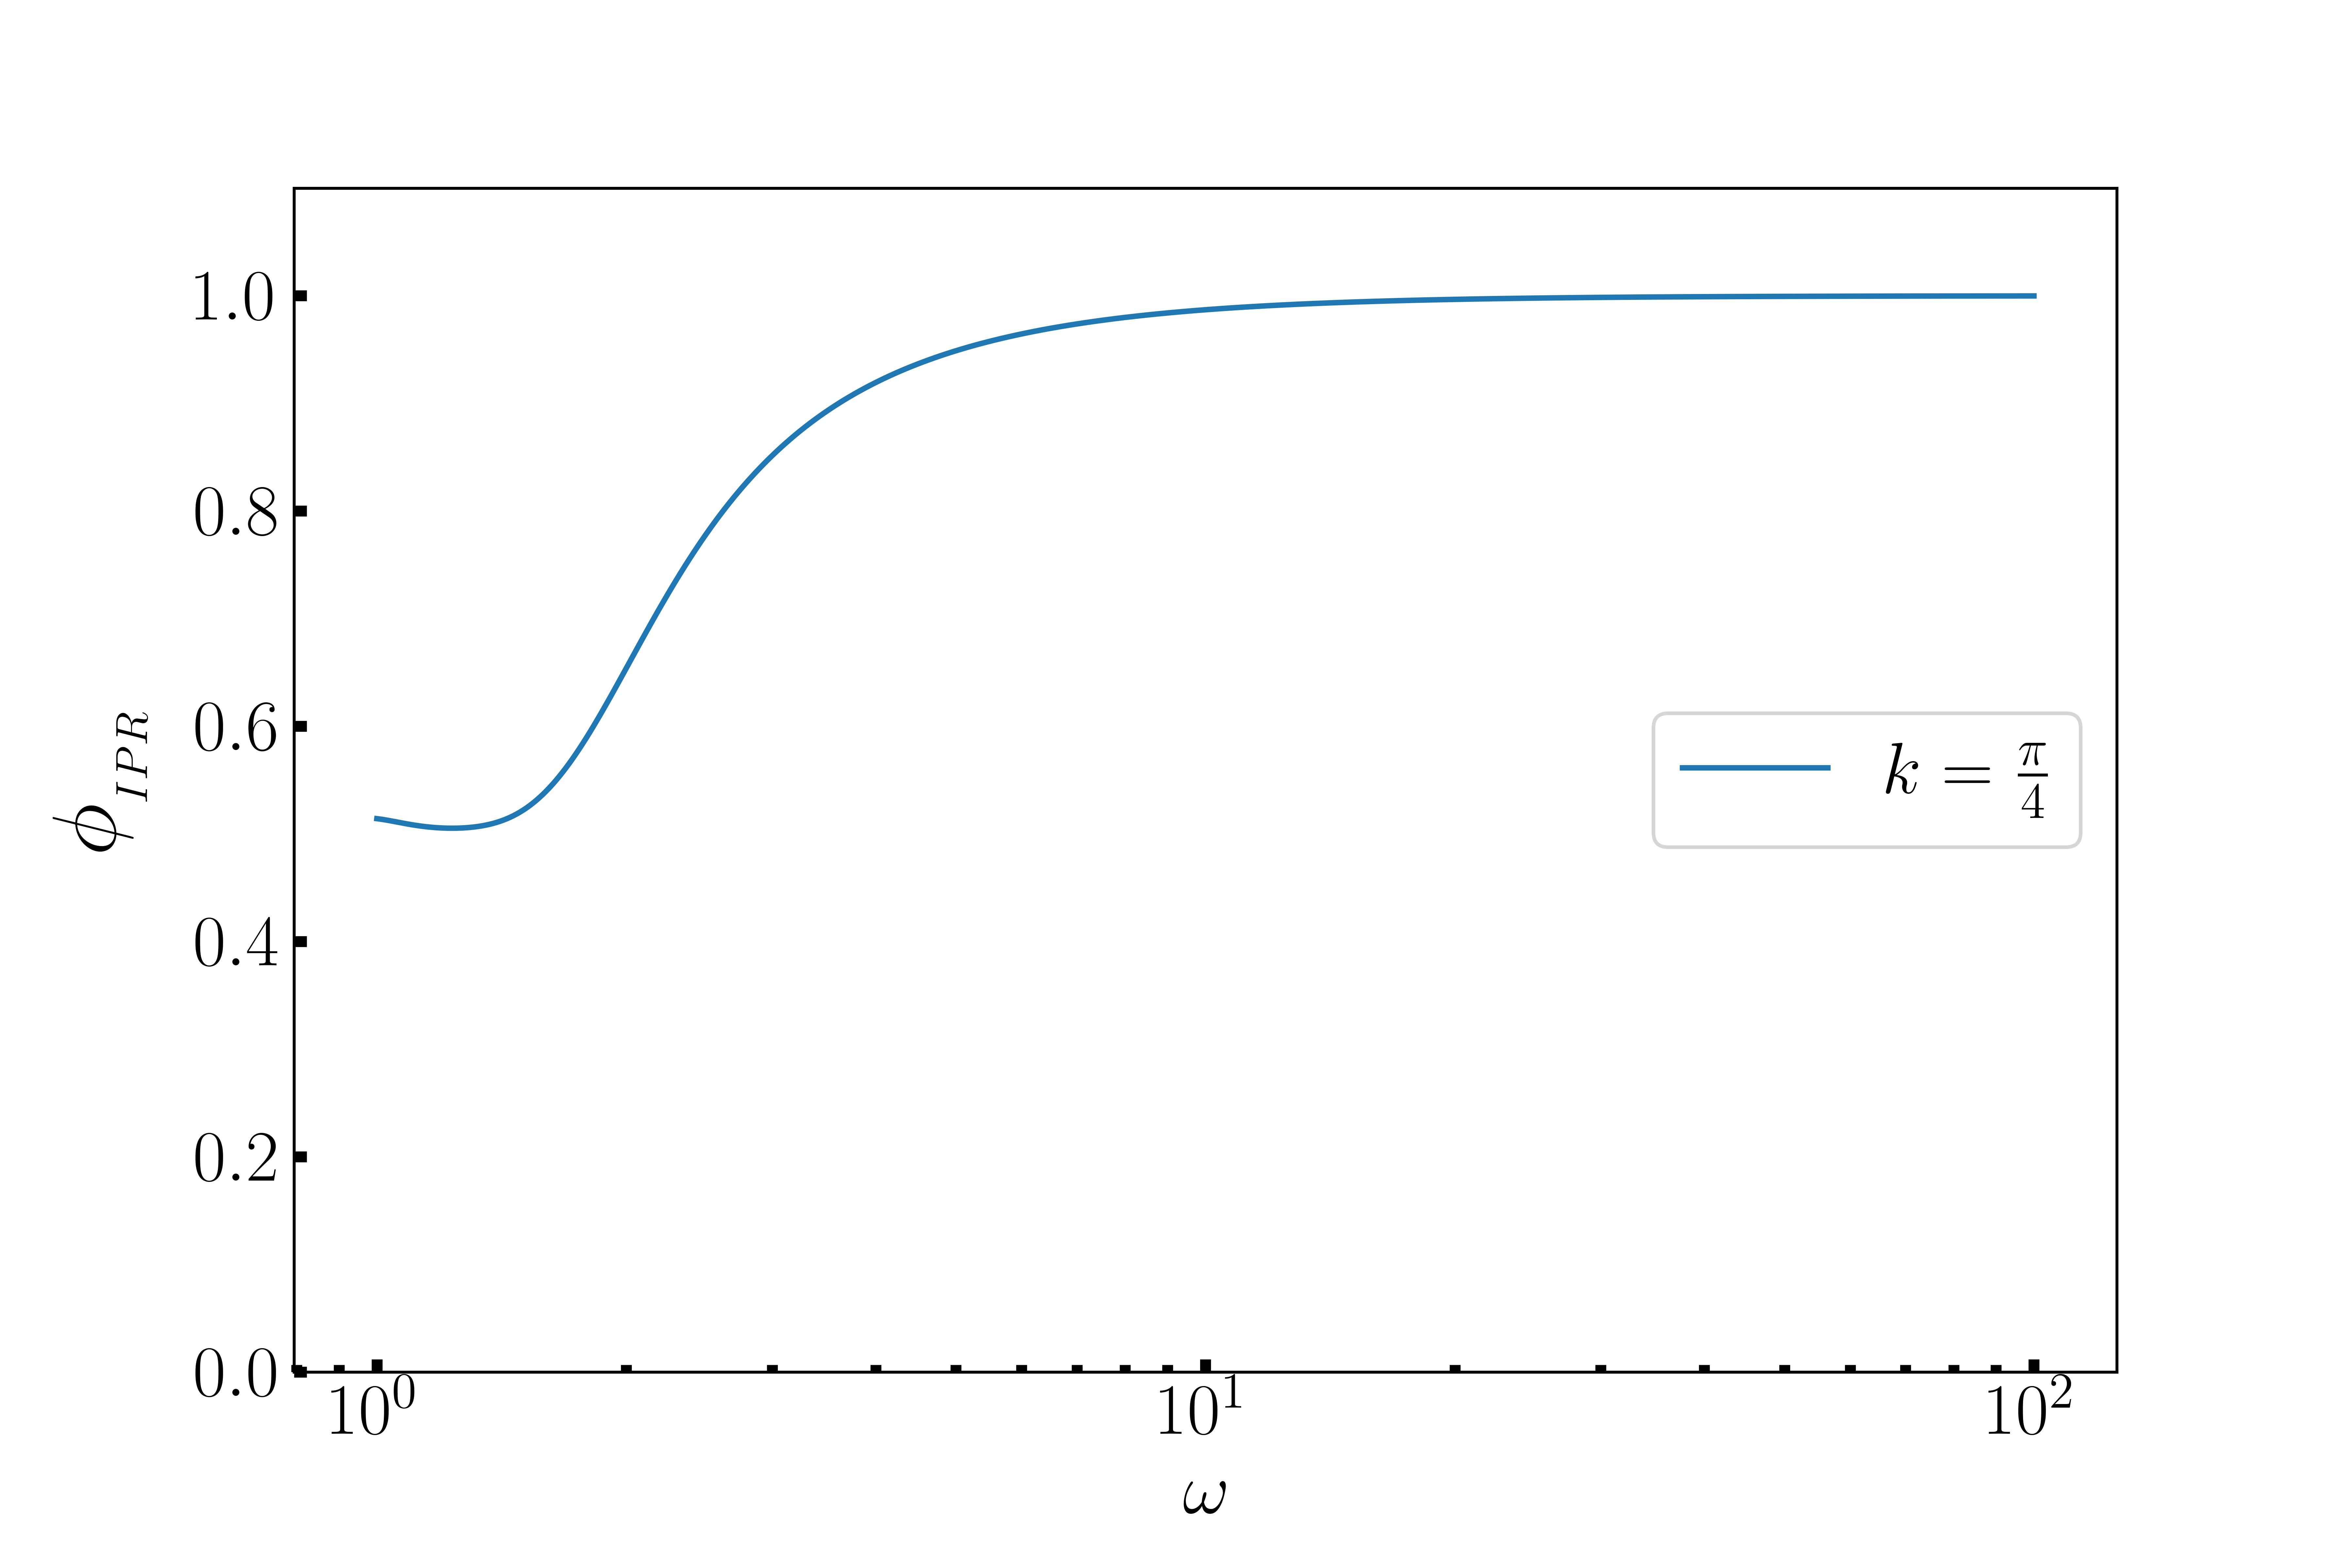
\includegraphics[height = 6cm, width = 9.0cm]{phase_transition_ising.jpeg}
		\caption{IPR for TFIM is approximately 0.5 at lower frequency and 1 at higher frequency. The slow change in IPR from minimum to unity over a large frequency range indicates the absence of a mobility edge and, consequently, the absence of a phase transition. In addition, at the point of resonance at low frequency the system does not go ETH-thematization is indicated by the existence of a finite IPR.}
		\label{fig:ipr:isinglowfr}
	\end{figure}
	
	
	\begin{figure}[]
		\centering
		\includegraphics[height = 6cm, width =9cm]{low_frq_exactN500_ipr.jpeg}
		\caption{A low-frequency regime $\omega$ = 2.0 plot for IPR for Ising model at four different density points for system size $N = 500$. IPR localization persists nonetheless.}
		\label{fig:ipr:isinglowfrk}
	\end{figure}
	
	Because the dependence of observable expectations on the eigenstates is always fairly strong for integrable systems like the TFIM, such systems will never exhibit any kind of thermal behaviour unless integrability breaking terms are included. As a result, it is not physically meaningful to refer to this as "Many Body Localization," because the parameter space lacks a region where ETH holds to contrast with this state. The type of Floquet Engineering described above, on the other hand, can be easily applied to a broad class of nonintegrable systems where ETH is expected to hold in certain regions. Long-range spin systems, in particular, where the exchange energies between far-off spins are taken into account in the model Hamiltonian, are good candidates because they are known to thermalize when driven with low frequencies~\cite{russomanno_thermalization_2015}.
	\section{\label{sec:level3}Lipkin Meshkov Glick Model: Long range interaction}
	
	PROOFREAD FROM HERE!!!
	
	FROM HERE ON OUT, PLZ USE THE PHYSICS LATEX PACKAGE!!!
	
	
	Consider the Hamiltonian of the type
	\begin{equation}
	\hat{H}(t) = \hat{H}_0 + \left(h \cos{(\omega t)} + h_0\right)\; \hat{H}_1
	\label{eq:lmg:ham}
	\end{equation}
	where
	\begin{eqnarray*}
		\hat{H}_0 &=& \frac12 \sum_{ij}J_{ij}\hat{\sigma}^z_i\hat{\sigma}^z_j,\\
		\hat{H}_1 &=& \sum_i\hat{\sigma}^x_i.
	\end{eqnarray*}
	here,
	\begin{equation*}
		J_{ij} =\frac{J_\alpha}{N^{1-\alpha}}\frac{1}{r_{ij}}.
	\end{equation*}
	Putting  $\alpha = 0$ yields the Lipkin Meshkov Glick (LMG) model with all-to-all interaction, yielding $J_{ij} = J_0/N$. We choose to maintain the extensivity of the interaction energy by enforcing the condition
	\begin{equation*}
		\frac{J_0}{N} \sum_{i\neq j}1=\frac{J_0}{N}\frac{N(N-1)}{2}=1\\
	\end{equation*}
	yielding the Kac-norm $J_0=2/(N-1)$. Here, we have $N$ spin-$1/2$ particles in a $1-$ dimensional lattice, and $i,j$ are site indices. The Hamiltonianin equation \ref{eq:lmg:ham} commutes with $P_{ij}$  with $P_{ij}$ defined as $P_{ij} = \displaystyle\frac{1}{2}(1+ \vec{\sigma}_i\cdot\vec{\sigma}_j)$. In addition $[S^2, H]=0$, therefore the $S^2$ is invariant of motion, where $S^2=\abs{\vec{S}}^2$ with $\vec{S}$ defined as, $ \vec{S}=S^x\hat{x}+S^y\hat{y}+S^z\hat{z}\equiv\frac12 \sum_i \vec{\sigma}_i$. We now choose to populate the system in a state whose  measured value of $S^2$ is $\displaystyle\frac{N}{2}\left(\frac{N}{2}+1\right)$, in that case the dynamics remains invariant in the space spanned by the common eigen states of $P_{ij}, \abs{S}^2$ and $S_z$, these are also eigenstates in the so-called TSS subspace ~\cite{mori_prethermalization_2019}. Let the eigenvalues be $s_n$, and the eigen vectors be $\ket{s_n}$, where $s_n=-\frac{1}{2}+\frac{n}{N}$ and the index
	$n= 0 (1) N$ has $N+1$ values. So, the dynamics is restricted to a (N$\times$N) invariant subspace where the matrix elements are given by 
	
	\begin{align}
		(H_0)_{ij} &= -\frac{4}{N-1} s^2_i \delta_{ij},\nonumber\\
		(H_1)_{ij} &= \Bigg[\sqrt{\frac{N}{2}\left(\frac{N}{2}+1\right) - Ns_i\left(Ns_{i + 1}\right)}\delta_{i+1, j} \nonumber\\ 
		&\hskip 0.7cm +\sqrt{\frac{N}{2}\left(\frac{N}{2}+1\right) - Ns_i(Ns_{i- 1})}\delta_{i-1,j}\Bigg]
		\label{eq:lmg:tssham}
	\end{align}
	Now we transform the Hamiltonian to the Rotated frame given by the transformation
	
	\begin{equation}
	\hat{U}(t)=\exp [i \frac{h}{\omega} \sin (\omega t) \hat{H}_{1}]
	\end{equation}
	Defining $\tau = \displaystyle\frac{h}{\omega}\sin{\omega t}$, we use the fact that $\hat{H}_1 = 2 S^x$, and the identity  
	\begin{equation}
	e^{i 2\tau\hat{S^{x}}} \hat{S^{z}} e^{-i 2\tau \hat{S^{x}}}=\hat{S^{z}} \cos \left(2\tau\right)+\hat{S}^{y} \sin \left(2\tau\right)
	\end{equation}
	to simplify the transformed Hamiltonian, yielding
	
	\begin{align}
		\tilde{H}(t)& = -\frac{1}{N-1}\Big[\big(S^z\big)^2 \big(1+\cos{4\tau}\big)+ \big(S^y\big)^2 \big(1-\cos{4\tau}\big)\nonumber \\  
		&\hskip 2.5cm + \big\{S^y, S^z\big\}\sin{4\tau}\Big] - 2 h_0 S^x
	\end{align}
	
	
	We define $\eta\equiv 4h/\omega$ and use the Jacobi-Anger formulae ~\cite{arfkenmath}
	
	\begin{align*}
		\cos(\eta \sin\omega t) &= J_{0}(\eta)+2 \sum_{n=1}^{\infty} J_{2 n}(\eta) \cos (2 n \omega t) \\
		\sin(\eta \sin\omega t) &= 2 \sum_{n=1}^{\infty} J_{2 n-1}(\eta)\sin [(2 n-1) \omega t]
	\end{align*}
	to simplify the expression for $\tilde{H}(t)$. Finally, we assume that the drive frequency $\omega$ is large enough that all harmonic terms in the Hamiltonian can be averaged out over discernible time scales. This yields the Hamiltonian in the Rotated Wave Approximation (RWA) to be (ignoring constant terms in the addition)
	
	\begin{equation}
	\tilde{H}_{\mathrm{RWA}}= \frac{\big(\hat{S}^x\big)^{2}}{N-1} - 2h_0 \hat{S}^x - \frac{J_0(\eta)}{N-1}\bigg[\big(\hat{S}^z\big)^{2} - \big(\hat{S}^y\big)^{2} \bigg]
	\end{equation}
	
	
	If the drive amplitude $h$ is adjusted such that $\eta$ lies at a root of $J_0(\eta)$ (the localization point), the RWA Hamiltonian is diagonal in the representation of the transverse field $\hat{S}^x$, yielding an IPR of unity in that representation, similar to the Ising case. Note however, that if the DC transverse field $h_0$ is set to $0$, then, at the localization point, the RWA Hamiltonian $\tilde{H}_{\mathrm{RWA}}\sim
	\big(\hat{S}^x\big)^2$, each of whose eigenvalues (given by $\big(\frac{N}{2}-m\big)^2$ where $m \in 0(1)N$, and $\big(\frac{N}{2}-m\big)$  are the eigenvalues of $\hat{S}^x$) are two-fold degenerate. This produces infinitely many (Floquet) eigenmodes in the degenerate subspace whose IPRs may not always be unity in the $S^x$ representation. Thus, the absence of the DC field may produce delocalization in the Floquet states even at the localization points, and this necessitated the inclusion of a DC field $h_0$ in order to break the symmetry.
	Finally, note that not all values of the DC field $h_0$ remove all degeneracies in $\tilde{H}_{\mathrm{RWA}}$. To see this, note that, at the localization point, the eigenvalues of $\tilde{H}_{\mathrm{RWA}}$ are given by
	
	\begin{equation}
	\rm{Eigs}\bigg[\tilde{H}_{\mathrm{RWA}}\bigg] = \frac{\big(\frac{N}{2}-m\big)^2}{N-1} - 2h_0 \bigg(\frac{N}{2}-m\bigg)
	\end{equation}
	
	In order to ensure that no degeneracies occur, we have to adjust $h_0$ to ensure that for any two integers $m_1, m_2 \leq N$  the condition following is always met,
	
	\begin{equation}
	\frac{\big(\frac{N}{2}-m_1\big)^2}{N-1} - 2h_0 \bigg(\frac{N}{2}-m_1\bigg) \neq \frac{\big(\frac{N}{2}-m_2\big)^2}{N-1} - 2h_0 \bigg(\frac{N}{2}-m_2\bigg)
	\end{equation}
	
	If $N\gg 1$ (substantially large), then this condition can be met by assuring that $(1-2h_0)^{-1}$ is never an integer that is divisible by $N$. To ensure this in our numerical simulations we have kept $h_0$ at a small irrational value.
	
	
	This result is tentatively supported by exact simulations, as can be seen in the plots below in FIG. \ref{lmg_ipr_exact}. There, we show plots of the IPR of the Floquet mode $\ket{\phi^n}$ for all $n$ corresponding to eigenvalues of $S^x$ for a fixed eigenvalue of $S^2 = N/2\big(N/2 + 1\big)$. The IPR is thus
	\begin{equation}
	\phi_{IPR}(n) = \sum_m \abs{\ip{m}{\phi^n}}^4
	\label{iprlmg}
	\end{equation}
	where $|m\rangle$ is the $m^{th}$ eigenstate of $\hat{S}^x$.
	
	
	Now, we focus at numerical simulations for $H(t)$ via the IPR of the Floquet state in the representation of the transverse field i.e. the eigenstates of $S^x$. We kept $\omega = 90$ as a large enough value for RWA to hold, and $N=\mathcal{O}(10^2)$ which our standard computational resources will allow. 
	
	\begin{figure}[ht!]
		\centering
		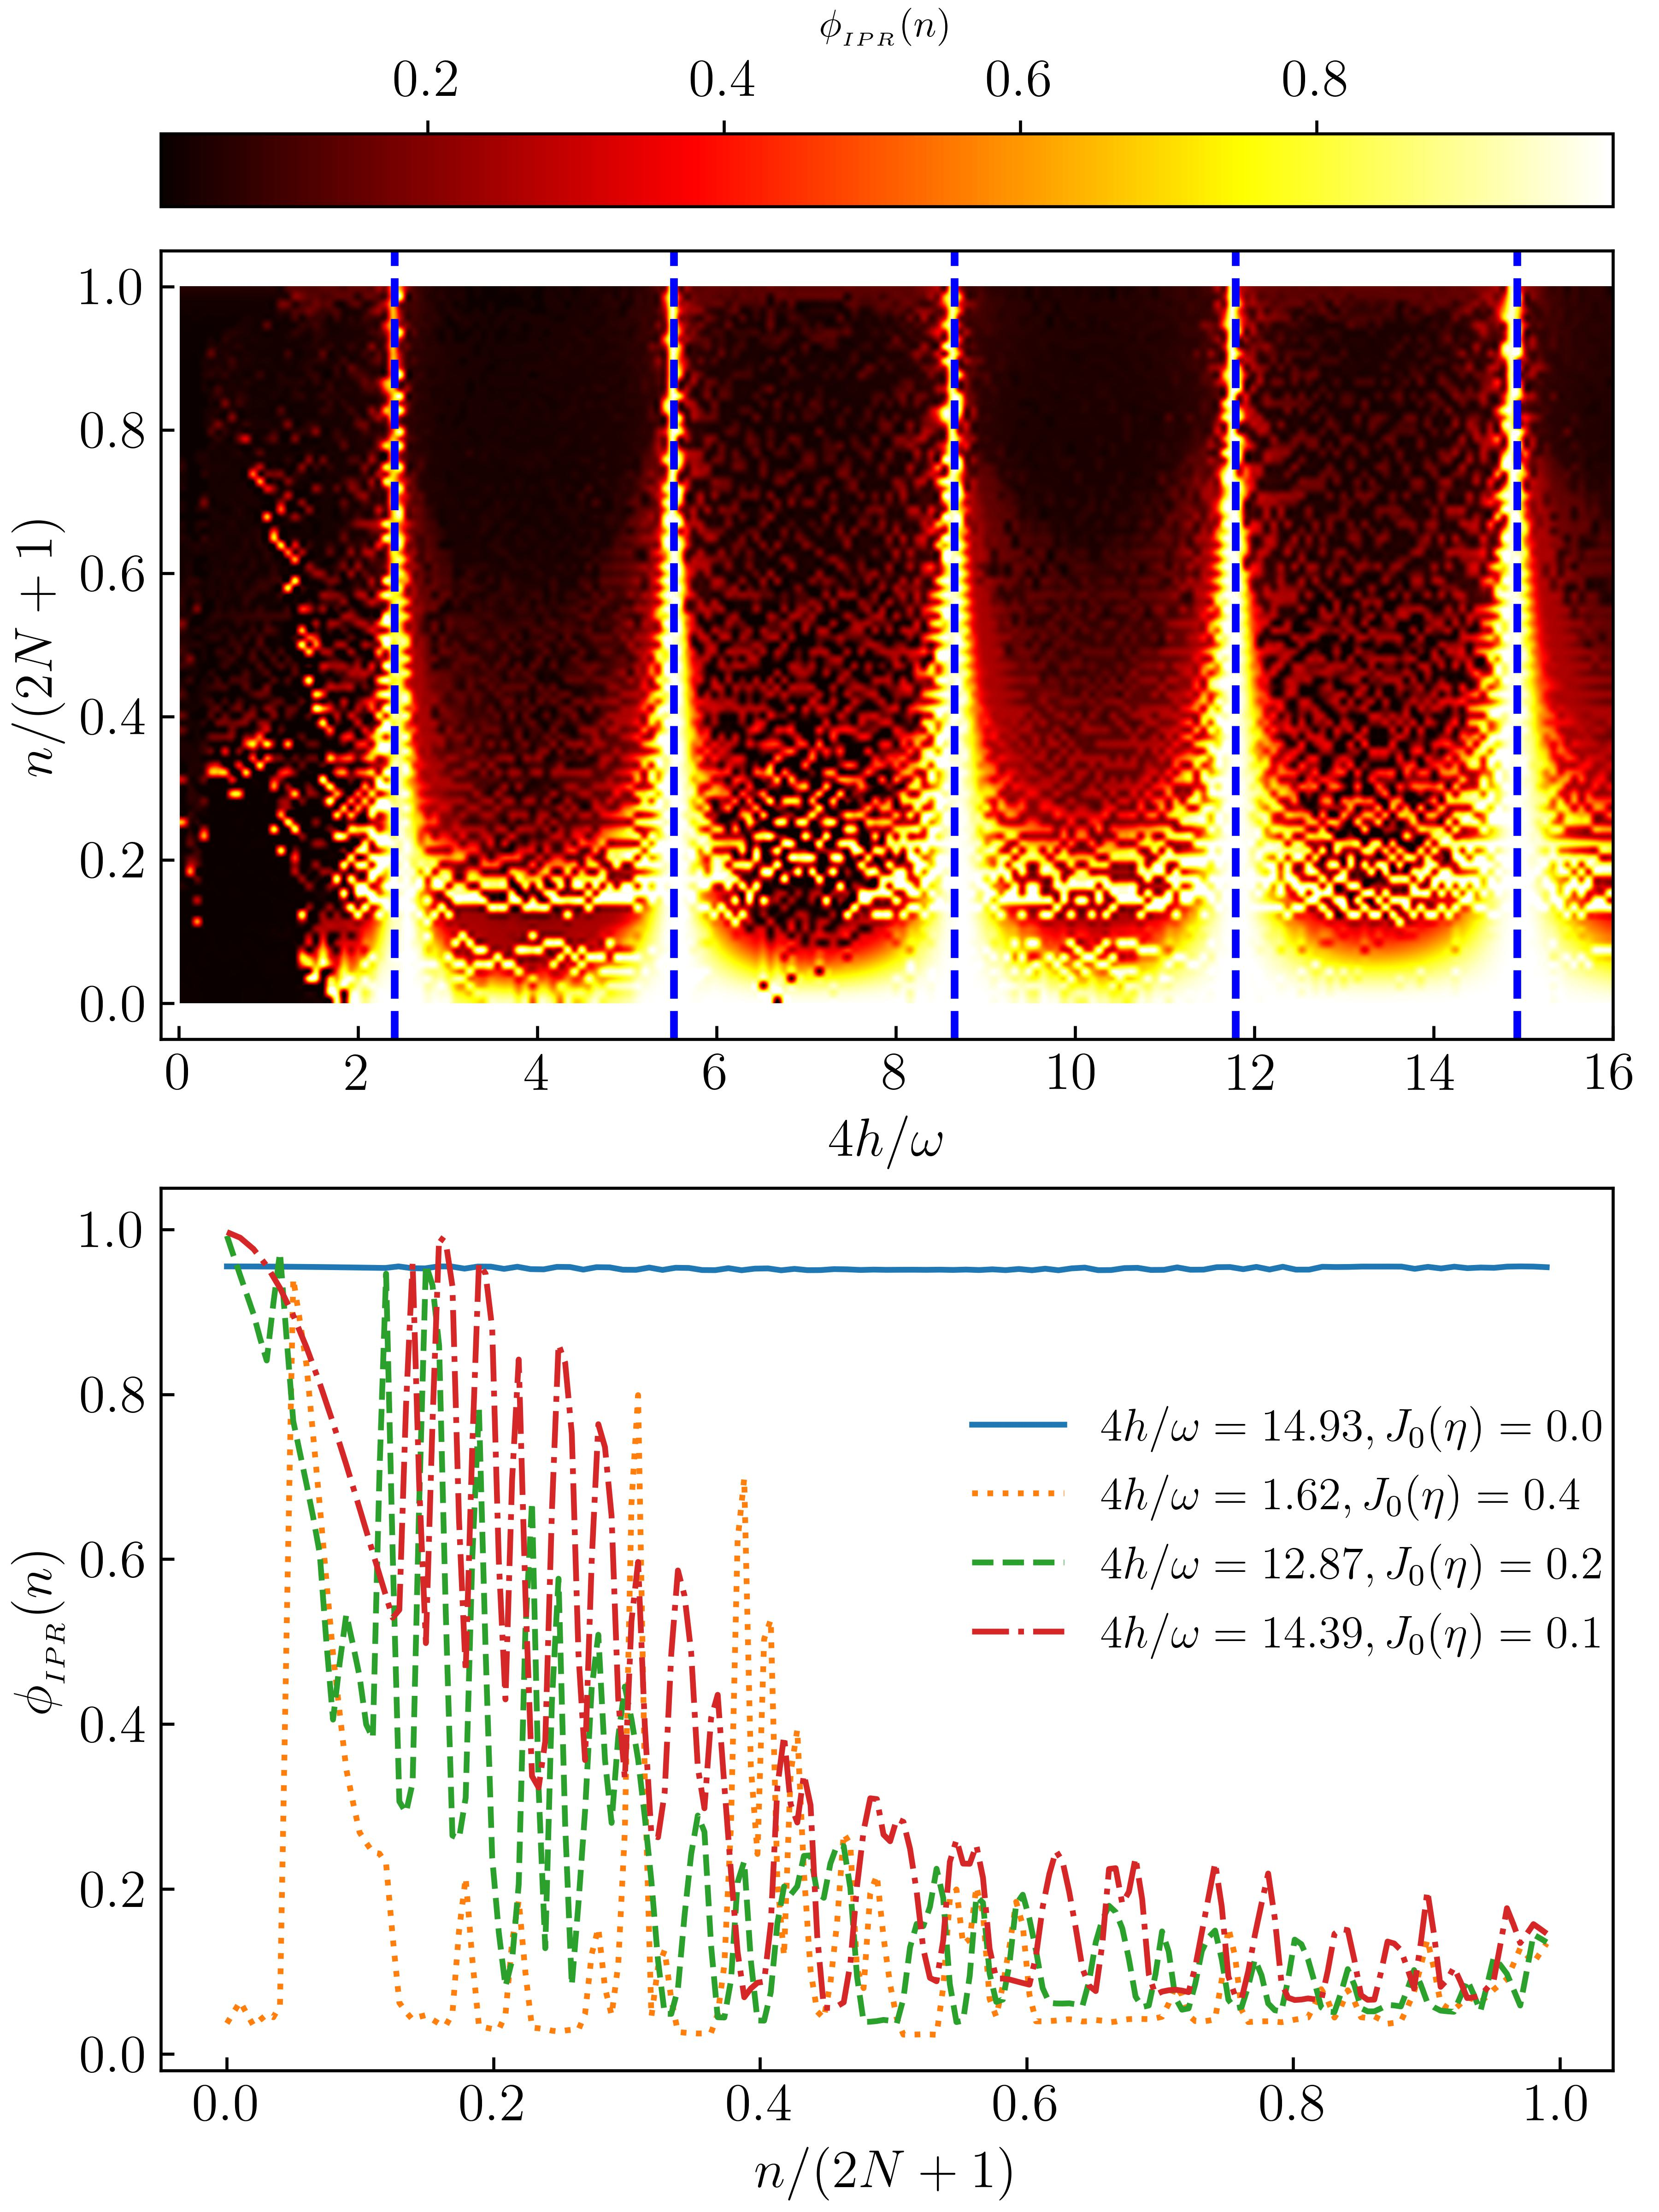
\includegraphics[height = 9.0cm, width =9cm]{ipr_exact_dynm_N50_frq_90_.jpeg}
		\caption{The IPR for exact dynamics for spin model size N$\sim$ 30. The upper panel shows a density plot of the IPR of Floquet modes for different parameter points corresponding to the ratio between strength and the frequency of the symmetry-breaking field which is the lowest root among Bessel's roots of the first kind and zeroth order $\frac{4h}{\omega}$. The dc part of the symmetry-breaking field is kept at a small irrational number to avoid the symmetry arising from degeneracy in Flqouet states. The IPR density is high at Bessel's first order roots, $J_0\Big(\frac{4h}{\omega}\Big)=0$ for all the available floquet states. The lower panel shows the crossectional plot of IPR for four different floquet IPR density points. The point corresponding $J_0\Big(\frac{4h}{\omega}\Big)=0$ has ~unity value for all states where points away from the roots have lower and high fluctuations.}
		\label{lmg_ipr_exact}
	\end{figure}
	The top panel has a density plot of the IPR of the Floquet states, with $\eta=4h/\omega$ on the abscissa and the spin index $m/(2N+1)$ on the ordinate. The dashed vertical lines (blue) correspond to roots of $J_0(\eta)$. As can be seen, the IPR is essentially unity at large roots of $J_0(\eta)$, indicating complete Many Body localization. However, there is some departure from unity at the smallest root of $J_0(\eta)$. This is due to the fact that at the smallest root of $J_0(\eta)\approx 2.405$, the amplitudes of the contributions of the higher order terms in the RW expansion, which are of $\mathcal{O}(J_n(\eta))$, are large enough to contribute to delocalization.
	
	The bottom panel contains cross sections of the full IPR plot for selected values of $\eta$ as indicated in the legend. When the drive amplitude $h$ is adjusted to make $J_0(\eta)\neq 0$, the Floquet States are mixed, but not entirely thermal, since the IPR does not fall to $\mathcal{O}(N^{-1})$, indicating that localization persists to some extent always.
	
	So, as long as there is an appropriate DC field, $S^x$ is mostly conserved and $H_F$ is mostly diagonal in the $S^x$ representation at the freezing point. The small deviations from this conservation occur due to the role of higher order terms in the Fourier expansion of the Hamiltonian on the rotating basis that contribute additional time-periodic terms to the RWA Hamiltonian, as can be seen in FIG.\ref{lmg_ipr_rwa}.
	
	The full Hamiltonian for the LMG model on the rotated basis is
	\begin{widetext}
		\begin{multline}
			\tilde{H}^{RWA}(t)\sim \frac{\big(\hat{S}^x\big)^{2}}{N-1} - 2h_0 \hat{S}^x - \frac{J_0(\eta)}{N-1}\bigg[\big(\hat{S}^z\big)^{2} - \big(\hat{S}^y\big)^{2} \bigg] - \frac{2}{N-1}\sum^\infty_{n=1}\;J_{2n}(\eta)\;\Big[\big( \hat{S}^z\big)^2 - \big( \hat{S}^y\big)^2\Big]\;\cos{\big(2n\omega t\big)}\\
			- \frac{2}{N-1}\sum^\infty_{n=1}J_{2n-1}(\eta)\;\big\{ \hat{S}^y,  \hat{S}^z \big\}  \;\sin{\Big[\big(2n-1\big)\omega t\Big]}
		\end{multline}
	\end{widetext}
	
	\begin{figure}[ht!]
		\centering
		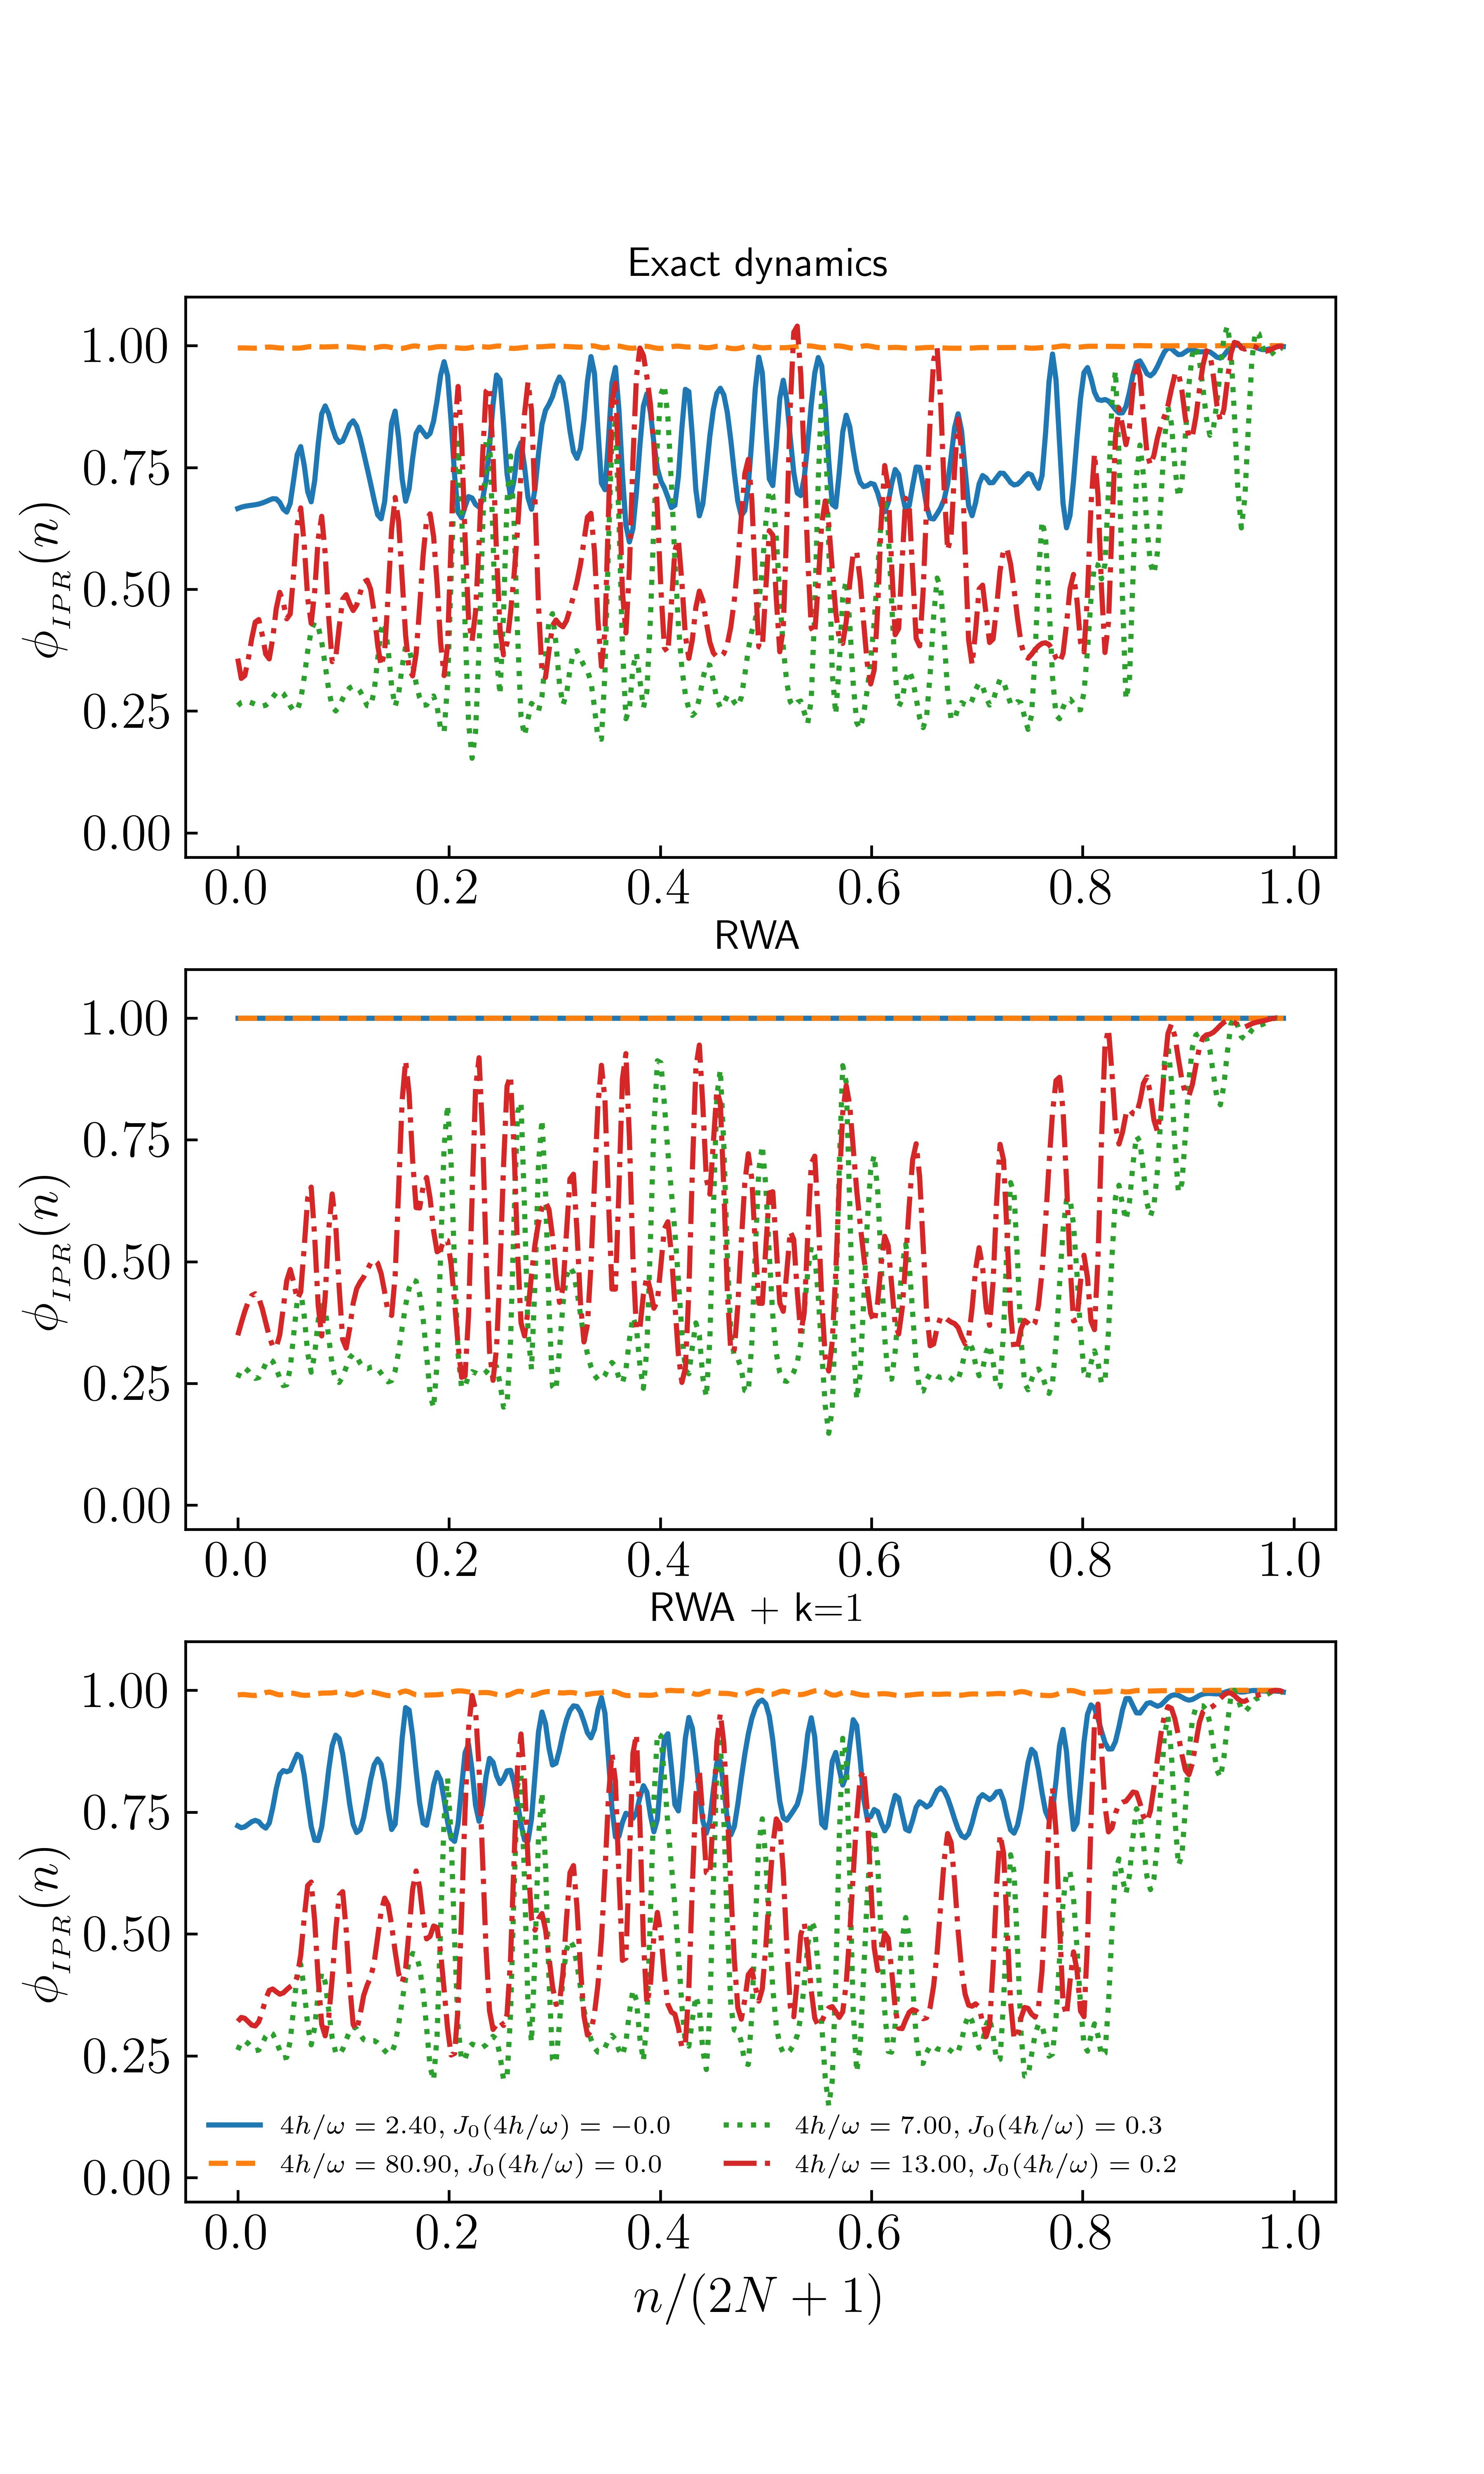
\includegraphics[height = 12.0cm, width =9.0cm]{comprasion_LMG_50_highFr90_exact_nd_rwa.jpeg}
		\label{lmg_ipr_rwa}
		\caption{The comparison between IPR for exact dynamics and RWA with corresponding correction orders. IPR is calculated for four different $\eta$'s and corresponding $J_0(\eta)\neq 0$ values. blue:$\eta = 2.40, J_0(\eta) = 0.0$, dashed orange:$\eta = 18.07, J_0(\eta) = 0.0$, green:$\eta =13.03, J_0(\eta) = 0.21$, red:$\eta = 1.62, J_0(\eta)= 0.44$. IPR plots for RWA with zeroth order aren't enough to describe the exact dynamics, but plots for RWA with first-order correction are similar to the exact dynamics.}
	\end{figure}
	
	IPR plots for precise dynamics describe that the freezing point at first (blue colour curve) Bessel's root of zeroth order of first kind is not enough for many-body localization in the top panel. This is because of the corresponding higher magnitude of other Bessel's roots of higher order. At higher localization points (shown in orange with dashes), many-body localization is most noticeable. Away from the point of localization, various curves, both green and red, represent how scattered the system is.	RWA for zeroth order in the centre panel has a nearly identical pattern at places that are further away from localization points (green and red), but the curves for both higher and lower localization points have fully localised, which contradicts the precise conclusion found in the panel on top. In the bottom panel, RWA which has been corrected to the first order exhibits a similar curve structure with exact dynamics.
	
	\section{\label{sec:level4}Classical Lipkin Dynamics}
	In the classical(continuum) limit, $N\rightarrow\infty$, we can ignore the difference between adjacent values of $s_i$ in equation \ref{eq:lmg:tssham}, and the Hamiltonian per particle becomes $h(t)\equiv \frac{1}{N}H(t) = h + h_0\cos{(\omega t)}h_1$, where
	\begin{eqnarray}
	(h)_{ij} &\approx& - 2s^2_i \delta_{ij},\nonumber\\
	H_0 &\rightarrow& -2s^2\\
	(h_1)_{ij} &\approx& \sqrt{1 - 4s^2_i}\left[\delta_{i+1, j}  + \delta_{i-1,j}\right]\nonumber\\
	H_1 &\rightarrow& \sqrt{1 - 4s^2_i}\cos{p},
	\end{eqnarray}
	
	In the continuum limit, the Lipkin system can be described by $p,q$ with corresponding Hamiltonian ~\cite{sciolla_quantum_2010}:
	\begin{equation}
	H = -2 q^2 - h(t)\;\sqrt{1-4q^2}\;\cos{p},
	\label{eq:class:ham}
	\end{equation}
	which yields the Hamiltonian dynamical system 
	\begin{align}
		\dv{q}{t} &= h(t)\sqrt{1-4q^2}\sin{p}\nonumber \\
		\dv{p}{t} &= 4q\bigg[1-\frac{h(t)\cos{p}}{\sqrt{1-4q^2}}\bigg]
		\label{eq:class:poinc}
	\end{align}
	
	We solved Hamiltonian \ref{eq:class:ham} using equations \ref{eq:class:poinc} to obtain position and moemntum coordinates $p,q$ and plotted in the Poincar$\acute{e}$ surface of section (PSOS) strobbed at each multiple of time period. A chaotic Poincare pattern is found for all small drive amplitude $s.t.$  $A/J < 0.5 $ and also a regular pattern emerges at for ratios $A/J$ $\geq$ 0.5 both at small drive frequency $\omega \sim 2.0$ ~\cite{russomanno_thermalization_2015}. 
	
	But at a sufficient high-frequency regime, the system behaves differently. We have compared  Poincare sections of the ensuing dynamics for $h(t)=h\cos{\omega t}$ for two cases, one for which $\omega=2.5$ (smaller frequency and consequently small amplitude) and one at $\omega=90.0$ (high frequency and corresponding high amplitude) at $J_0(4h/\omega)=0$. These are compared with the Husimi Q-functions of the obtained Floquet States. The quantum phase space is described by the Spectral Average of the Husimi functions of all the Floquet modes $|\phi^n\rangle$ for the chosen value of $S^2$, i.e. for a coherent state $|q, p\rangle$, we plot in FIG. \ref{fig:classical_lipkin}.
	\begin{equation*}
		H(q,p)\equiv \frac{1}{\big(2N+1\big)\pi}\sum_n \ip{q,p}{\phi^n}\ip{\phi^n}{q,p}
	\end{equation*}
	
	At small $\omega$, where the classical plots are chaos dominated ~\cite{Kidd2019}, and at large $\omega$ the sharp regular pattern proves localization in the Poincar$\acute{e}$ plot. 
	\begin{figure}[ht!]
		\centering
		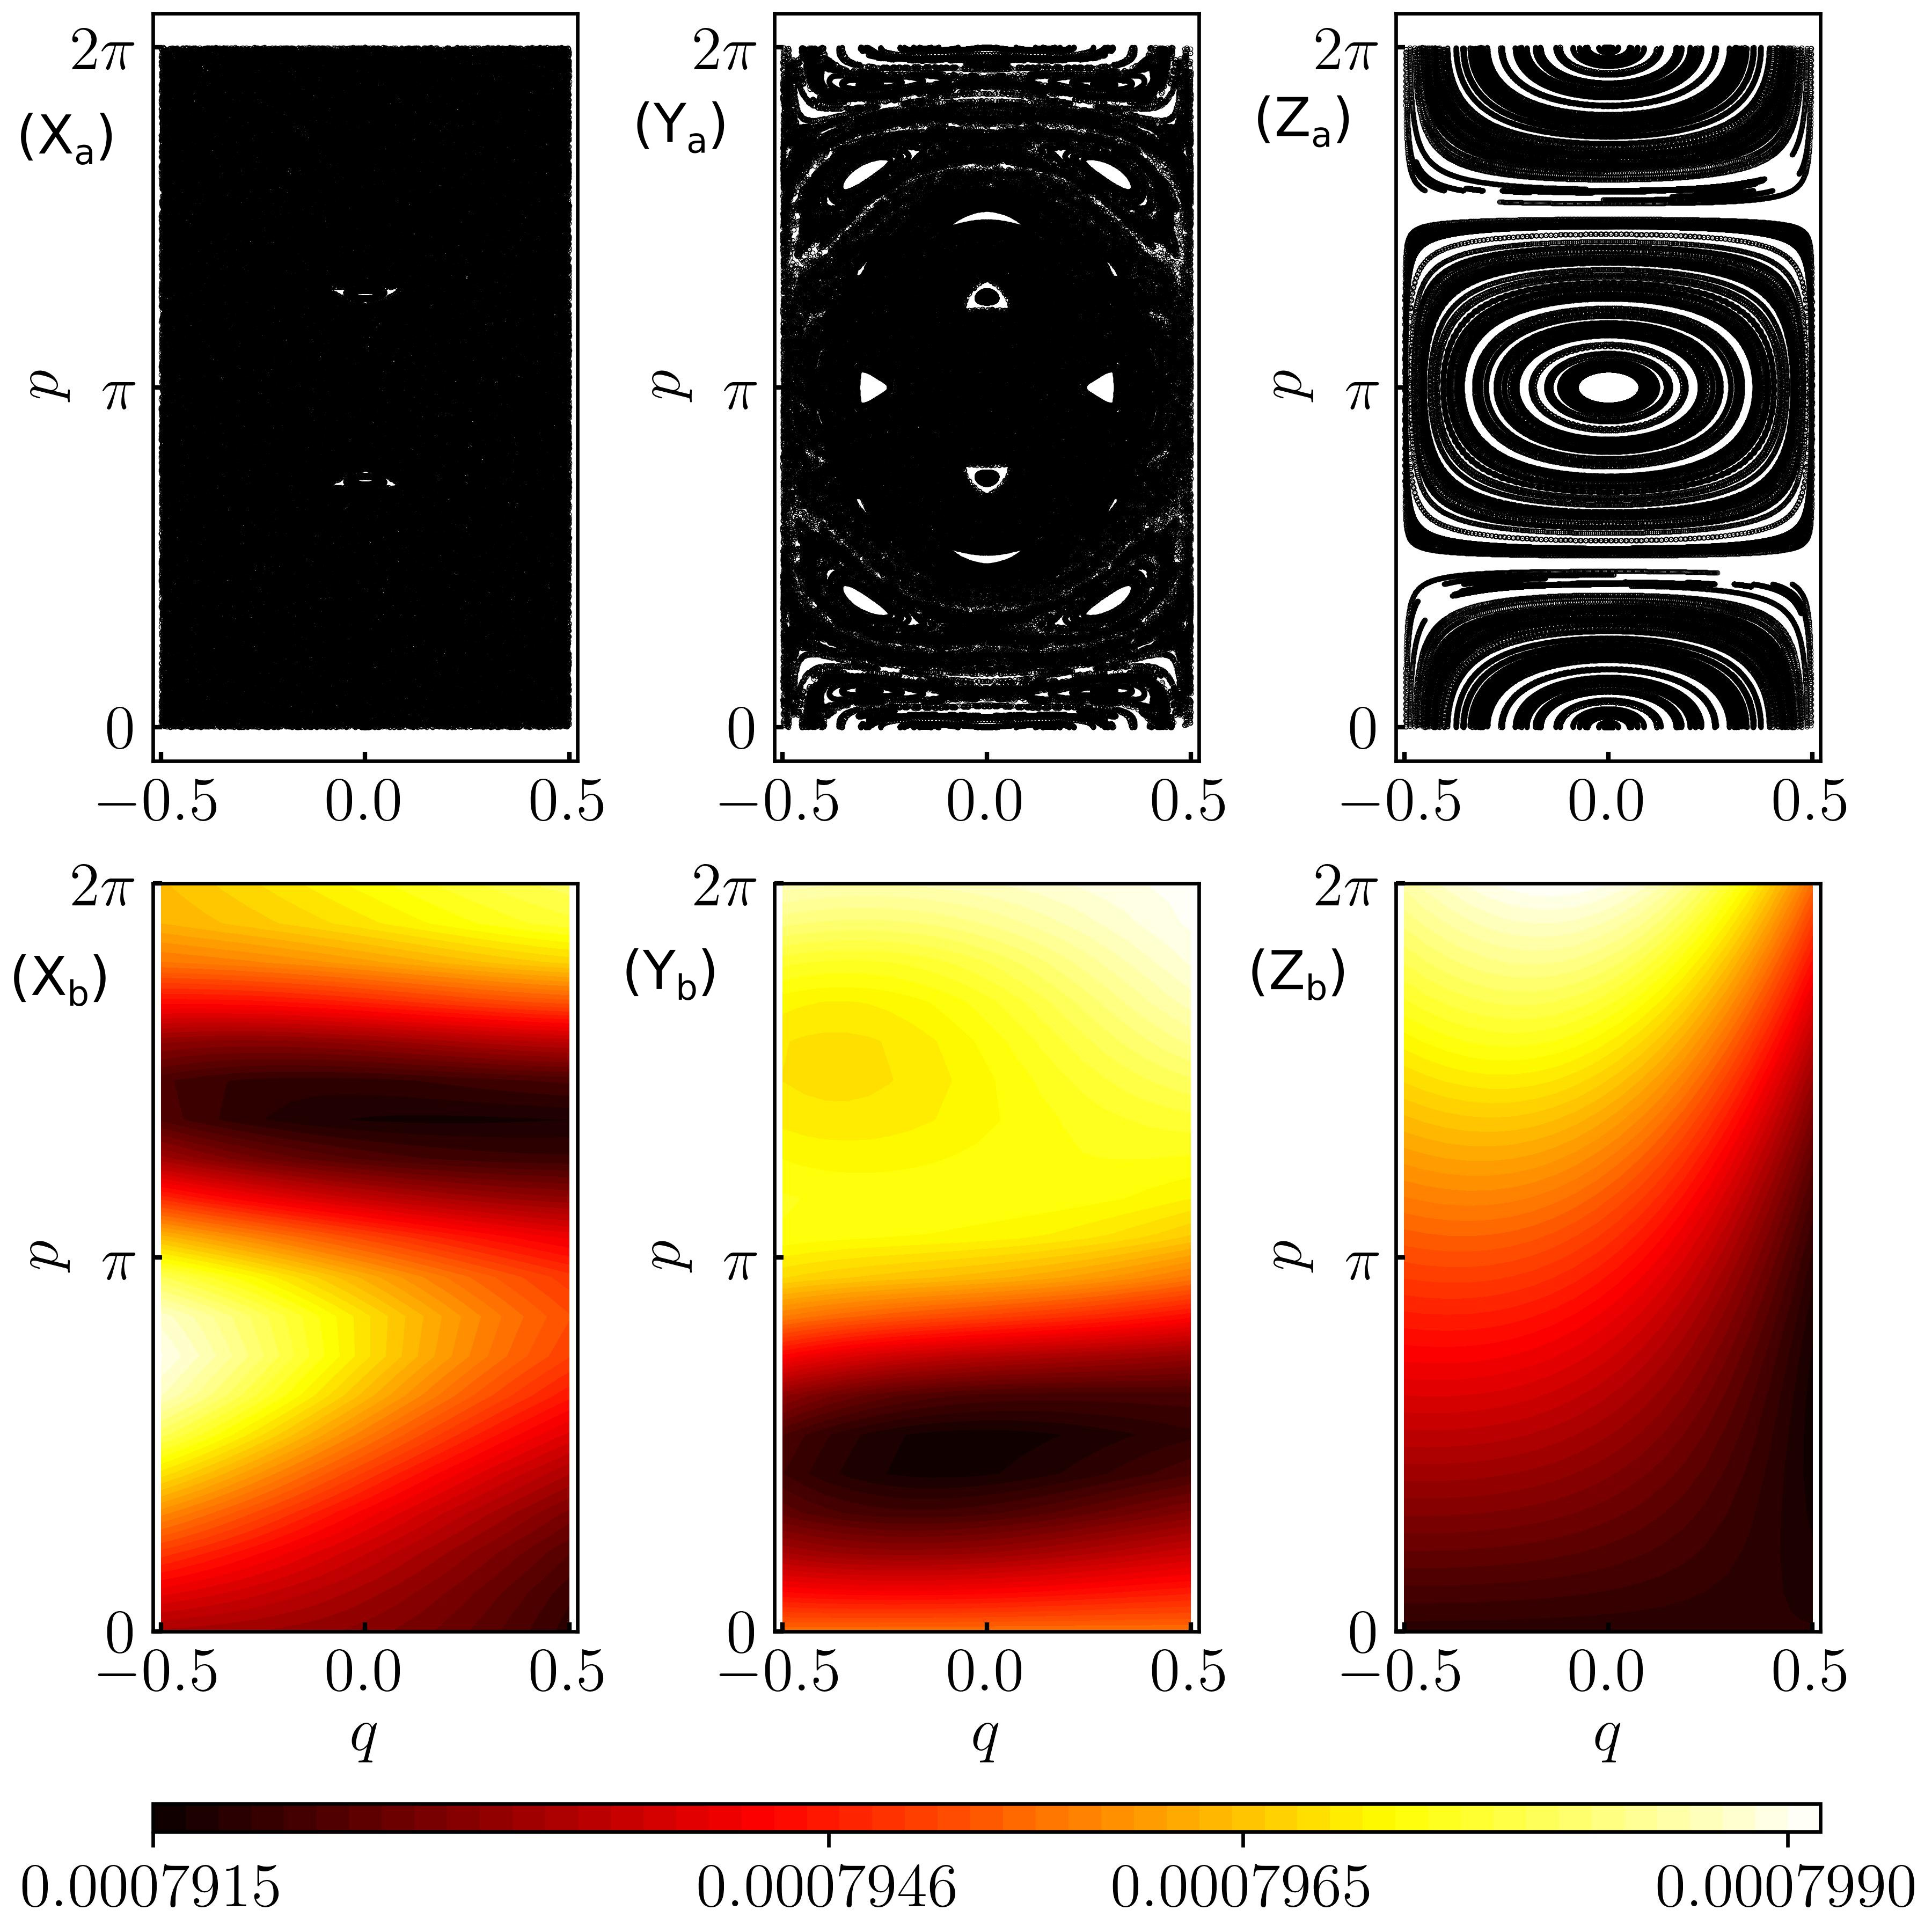
\includegraphics[height = 9.0cm, width = 9.0 cm]{lmg_poincare.jpeg}
		\caption{The above panel describes the phase-space Poincare distribution symmetry breaking smaller drive frequency $\omega = 2.5$ (left) and higher frequency $\omega = 90.0$ (right) for system size $N=500$ with 100 realisation numbers. At smaller frequencies, the Poincare picture contains chaotic behaviour (top left panel) whereas at the higher frequencies, it is a normal Poincare picture which represents discrete freezing behaviour(top right panel). The bottom panel is Hushimi Q-function average plot for  a smaller frequency (bottom left) and has a uniform distribution with less contrast in colour. This means a Q-function distribution in chaotic behaviour. At the right bottom, the Hushimi plot has distinct colour contrast in the Q-function average value which represents a regular dynamics pattern in the system.}
		\label{fig:classical_lipkin}
	\end{figure}
	\section{\label{sec:level5}Thermality to Athermality: A Phase Transition}
	So far, the dynamics of the Lipkin-Glick-Meshkov model exhibit two distinct scenarios at low and high external drive frequencies; hence, we propose there may be a frequency-induced phase shift. IPR of the floquet modes is computed numerically and plotted in FIG.\ref{fig:phase_transition} for numerous frequencies in ascending order from frequency $\omega = 1.0$ upto $\omega=50.0$ so that the system can grow adiabatically, along with the associated drive amplitude $h$ for the first of the localization point, which is $J_0\big(\frac{4h}{\omega}\big)$. (Top panel) At low-frequency region from $\omega =  1.0$ upto $\omega \sim 9.0 $, IPR is lower than unity and it gradually decreased as the system size increases which is $\frac1N$ variation of IPR which confirms the distribution of participation(Bottom panel). When $N\rightarrow \infty$ IPR appears to be zero which is fully delocalized state. At frequency $\omega \sim 9.0$ there is a sharp rise in IPR plot and IPR remains almost unity (Top panel) for higher frequencies even at change in system sizes. The sudden rise in IPR at frequency confirms phase transition in the frequency domain for LMG long-range spin model. 
	
	\begin{figure}[!ht]
		\centering
		\includegraphics[width = 8.8cm, height =9.0cm]{phase_transition_LMG_N.jpeg}
		\caption{For different spin sizes, $N = 10,20,30,50,100$, IPR is plotted at  Bessel's first root with first kind $J_0\Big(\frac{4h}{\omega}\Big)$ varying both the drive amplitude and frequency in LMG spin array. The drive frequency is increased adiabatically from sufficiently low-frequency O(1) and  up to high-frequency O(50) for system size N = 10,20,30,50,100 IPR found to be low enough at a small frequency up to a critical frequency where IPR rises to unity abruptly for each system sizes(Top panel).  It is also found that at low-frequency regions the system IPR decreases in the scale of N which confirms the distribution of participation of the states of the system (Bottom panel). The change in IPR at critical frequency is sharper as system size increases more, this indicates at infinite large system $N\xrightarrow{}\infty$ the change in IPR to unity is instantaneously resulting in a phase transition at critical frequency.}
		\label{fig:phase_transition}
	\end{figure}
	
	
	\section{\label{sec:level6}Observations and Discussion}
	
	For ising model quantum many-body localization is present at high drive frequency and corresponding high drive amplitude at localization points obtained by fixing $J_0(2h/{\omega}\big)=0$ for both exact and Rotated wave simulations with fairly weak delocalization away from the localization points. Since the Ising model is integrable, localization can be observed even at tiny $\omega$ values, despite the fact that RWA breaks out and analytical approaches beyond the adiabatic limit are complex. In the LMG model, we can see clear localization at localization points, obtained by fixing $J_0(4h/\omega)=0$, for both the exact and Rotated Wave simulations, with fairly weak delocalization away from those points. Due to the fact that the LMG model is non-integrable and the start of chaos in the thermodynamic limit for small $\omega$ is well-known, we can witness near full delocalization in the IPR of the Floquet states for tiny $\omega$. 
	
	Consequently, we adiabatically varied $\omega, h$ in the LMG model, under the constraint that $\eta=4h/\omega$ was held at a root of $J_0(\eta)$. There, we observed a crossover or phase change from nearly fully thermal to completely localised behaviour (see FIG.\ref{fig:phase_transition}).
	Even if the limitation is relaxed, the macroscopic behaviour changes from thermal to athermal.
	At low frequencies, IPR is observed to decrease with increasing system size N, and when N is big, i.e., $\rightarrow{} \infty$, IPR appears to evaporate, resulting in a fully thermalized state at $\eta=4h/\omega$.
	This is in contrast to the Ising model, which lacks such a transition.
	Thus, the incorporation of long-range interactions appears to trigger a transition from the thermal phase to the localised phase, a property that will prove useful in the design of MBL engines. 
	
	\section{\label{sec:level7}Conclusion and Outlook}
	
	As a paradigmatic example, we explored the beginning of Dynamical Many-Body Localization in regularly driven long-range spins for the Lipkin-Glick-Meshkov spin model. The many-body localization is parametrized by the Inverse Participation Ratio of the Floquet eigenstates. We numerically compared the IPR of the LMG model to that of the TFIM for low and high drive frequencies. We also investigated the LMG model's phase space dynamics to analyse the advent of thermal behaviour at low frequencies and localization at high frequencies, as well as the onset of additional approximately conserved quantities in the high-frequency regime for both models. 
	
	\emph{Conclusion}: Long-range spins exhibit strong localization in spin-coordinate space for the LMG model when the drive frequency is $\omega \gg J$, where $J$ represents the spin exchange energy. For the LMG model localization takes place at particular resonances of the drive frequency $\omega$ and amplitude $h$, $\textit{i.e.}$ when $J_0(4h/\omega)=0$. While similar localization (in momentum space) has been observed for the TFIM case at resonances given by $J_0(2h/\omega)=0$, the mechanism is different in long-range systems due to the conservation of a different observable $(S_x)^2$ in the LMG case, where $\mathbf{S}$ is the total spin. Once the accidental degeneracy is eliminated by a DC transverse field of the form $\sim \hat{S_x}$, the eigenstates can be mapped to a coordinate representation, resulting in robust spatial localization. A strong mobility edge is also seen in the periodically driven LMG model as the frequency is increased adiabatically from $\omega \sim J$ to $\omega \gg J$.
	In the first regime, the quantum system will thermalize at infinite temperatures because the classical dynamics will have entered a state of dynamical chaos.
	But in the latter regime, this is perpetually postponed due to dynamical localization. The mobility edge between these regimes shows singular behaviour in the thermodynamic limit, suggesting a quantum phase transition between them. This is not present in the short-range TFIM, where the IPR is too large in the low-frequency limit to induce thermal behaviour. Thus, Floquet engineering in long-range systems is sufficient to induce Thermal and MBL states, and disorder is not required.
	
	\emph{Outlook}: 
	We have examined a clean system with high symmetry. In all cases, thermalization occurs in addition to integrability-breaking terms (such as disorder), but similar to TFIM, thermalization should be delayed in LMG when at $\omega\gg J$ and $J_0(4h/\omega) = 0$. For systems with Hamiltonian $\mathcal{H} = -\frac{J_{ij}}{|i-j|^\beta} \sum_{ij}\sigma^z_i\sigma^z_j -\sum_i \sigma^x_i$, the less studied intermediate spin-spin interaction power law limits, i.e. $0<\beta<\infty$, rather than the infinite and long-range limit, can be studied further. The adiabatic increase in drive frequency causes a phase transition in the LMG spin configuration, indicating a future MBL engine with a thermodynamic cycle that operates between the thermal and MBL regimes. There are also opportunities for diabatic corrections. 
	
	
	
	{\it Acknowledgement:}
	One of the authors (MR) thankfully acknowledges The University of Burdwan for granting the state-funded fellowship.
	
	
	
	% The \nocite command causes all entries in a bibliography to be printed out
	% whether or not they are actually referenced in the text. This is appropriate
	% for the sample file to show the different styles of references, but authors
	% most likely will not want to use it.
	\nocite{*}
	
	\bibliography{main}% Produces the bibliography via BibTeX.
	
\end{document}
%
% ****** End of file apssamp.tex ******
